\section{Prüfung 02.02.2022}

\subsection{1. Echtzeit}
\subsubsection{a)}
Ein Profit/Penalty-Diagramm gibt den Nutzen bzw. den Schaden der Ausführung einer Operation als
kontinuierlichen Zahlenwert in Abhängigkeit vom Zeitpunkt der Ausführung an. Positive Werte
bedeuten einen Nutzen, negative einen Schaden – je größer der Absolutwert, desto größer der Nutzen
bzw. der Schaden.
Eine SPS mit einer Zykluszeit von 15 ms, einer Eingabezeit von 10 ms und einer Ausgabezeit von 5 ms
steuert eine Bremsanlage. Falls nach Betätigen des Bremshebels (als Sensor an die SPS angeschlossen)
mehr als 35 ms vergehen bis die Bremse (als Aktuator an die SPS angeschlossen) aktiviert wird, dann
kommt es zu einem Unfall. Die SPS wird zum Zeitpunkt 0 eingeschaltet, dann beginnt der erste EVADurchlauf und wiederholt sich dann periodisch alle 10+15+5=30 ms.
Zeichnen Sie in das Diagramm unten den Verlauf der Profit-Penalty-Funktion für die Operation
„Betätigen des Bremshebels“ ein.

\begin{figure}
  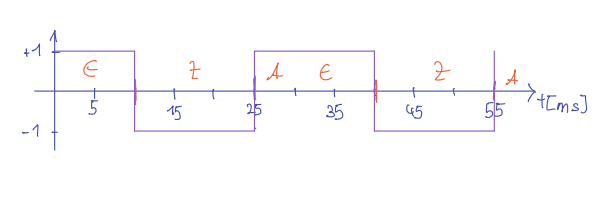
\includegraphics[width=10cm]{images/KA020222/1a.PNG}
  \centering
\end{figure}

\subsubsection{b)}
Handelt es sich hier um weiche, feste oder harte Echtzeit? Begründen Sie!

In diesem Beispiel handelt sich um harte Echtzeit. Wird der Bremshebel nicht betätigt wird es zu einem Schaden kommen.

\subsection{2. Echtzeitkommunikation}
\subsubsection{a)}
Nennen und erläutern Sie zwei wesentliche technische Unterschiede zwischen PROFInet SRT und
PROFInet IRT.

SRT = \textbf{S}oft \textbf{R}eal \textbf{T}ime wird für Prozess Automatisierung verwendet. Ist eine pure Software Lösung.
IRT = \textbf{I}sochronous \textbf{R}eal \textbf{T}ime wird für Motion Control verwendet. Ist eine Hardware Implementation  für Zyklus
synchronisation und Time slot control. Kleinere Zykluszeit und Jitter.

\subsubsection{b)}
Warum verwendet man bei Bluetooth „Frequency Hopping“?

